\section{\LangOO, The underlying programming language }  

\subsection{\LangOO syntax runtime configurations}
\label{sub:Loo} 
 \LangOO  is a {small}, imperative, sequential,  class based, typed, object-oriented language,  
 with private fields, private and public methods, unforgeable addresses, and no ambient authority (no static methods, no address manipulation).
 It has a simple concept of module with module-private fields and methods, described in Sect. \ref{sect:execution}.
 The definition of \LangOO  {can be found in the appendices  \cite{necessityFull}}, and is  similar to   OOPSLA-22.\footnoteSD{any differences?}

A \LangOO state, $\sigma$,  consists of a  heap $\chi$, and a   stack $\psi$. A stack is is a sequence of frames, $\phi$.
A frame consists of a local variable map, and a continuation, \ie a sequence of statements to be executed.


 
\paragraph{Notation} We adopt the following, unsurprising, notation:
\begin{itemize}
\item
$\alpha$, $\alpha'$, $\alpha_1$, ... are addresses,   $x$, $x'$, $x_1$, ..., $y$, ... $z$, ... are variables, and $\va$, $\va'$ ... are either addresses or variables, we call these \emph{\atoms}.
\item
$\alpha \in \sigma$ means that $\alpha$ is defined in the heap of $\sigma$, and $x\in \sigma$ means that $x$ is defined in the top frame of $\sigma$.

Conversely,  $\alpha\notin\sigma$ and $x\notin\sigma$ %, and $\va \notin A$ h
 have the obvious meanings.
\item
$\interpret{\sigma}{\alpha}$  is $\alpha$; and $\interpret{\sigma}{x}$  is the value to which  $x$  is mapped in the top-most frame of $\sigma$'s stack, 
and $\interpret{\sigma}{e.f}$ looks up in $\sigma$'s heap the value of $f$ for the object  $\interpret{\sigma}{e}$.
Note that $\interpret{\sigma}{e}$ is not defined when $e$ contains a method call or a ghost field.
\item The substitution  $\sigma[x \mapsto \alpha]$ is applied to the top frame of $\sigma$, and $\sigma[\overline{x \mapsto \alpha}]$ % applies the substitutions $\overline{x \mapsto \alpha}$ to the top frame.
has the expected meaning.
\item
$\sigma.\prg{cont}$ is the continuation in the top frame.
\item
$text_1 \txteq text_2$ expresses that $text_1$ and $text_2$ are textually equal.
\end{itemize}

  

  
\subsection{\LangOO Execution}
\label{sect:execution}

%Central to our work is the distriction between the 
 \LangOO execution is described by a small steps operational semantics of the shape $\leadstoOrig  {\Mtwo} {\sigma}   {\sigma'}$.\\
  $\Mtwo$ stands for one or more modules, where a
  module,  $M$, maps class names to class definitions. 
   
{The semantics enforces dynamically a simple form of module-wide privacy: 
Fields may be read or written only if the class of the object whose field is being read or written, and the class of the object which is reading or writing belong to the same module.}
Private methods may be called only if the class of the receiver (the object whose method is being called), and the class of the caller (the object which is calling) belong to the same module.
Public methods may always be called.

The semantics is as unsurprising in all remaining aspects  :  
In $\sigma$, the  top frame's continuation contains the statement to be  executed next.  
 Statements may assign to variables, allocate new objects, 
perform field reads and writes on objects, and
 call methods on those objects. 
When a method is called, a new frame is pushed onto the stack; this frame  maps \prg{this} and the formal parameters to  the values for the receiver and other arguments, and the continuation to the body of the method.  When the continuation is ground\footnoteSD{TODO check and define}, the frame is popped and the value from the last frame's continuation is entered into the appropriate part in the caller's continuation. 
%In other aspects, the semantics is unsurprisring.%we return from that call, its frame is  popped, and execution continues in the context of the calling method. 
%The relation $\leadstoOrigStar  {\Mtwo} {\_}   {\_}$  is the reflexive, transitive closure of $\leadstoOrig  {\Mtwo} {\_}   {\_}$ .


{Fig. \ref{fig:UpSemantics} illustrates  such  execution steps:  disks indicate states;
 horizontal $\leadsto$-arrows denote   steps  within the same  call; upwards arrows denote  method calls;
 %(pushing a new frame onto the stack);  
 downwards arrows denote method returns. % (popping the top of the stack). 
 Here,   $\leadstoOrig {\Mtwo}{\sigma_8}   {\sigma_9} $ is a step within the same call, $\leadstoOrig {\Mtwo}{\sigma_9}   {\sigma_{10}} $ is a method call   
with $\leadstoOrig {\Mtwo}{\sigma_{12}}   {\sigma_{13}} $ %is a method return  (from the call to $m_a$), 
the corresponding return. 
 {Note that  $\leadstoOrigStar  {\Mtwo} {\sigma}   {\sigma'}$ may involve  any number of  calls or returns: 
 $\leadstoOrigStar  {\Mtwo} {\sigma_8}   {\sigma_{12}}$ involves one call and no return,
while $\leadstoOrigStar  {\Mtwo} {\sigma_{10}}   {\sigma_{15}}$,   involves no calls and two returns.
% In section \ref{sect:bounded}, we will define a derived relation, called bounded execution, where the number of returns may not exceed the number of calls.
}
} 

\begin{figure}[htb]
\begin{tabular}{|c|}
 \hline %  \\ -- this added one vertical space
\resizebox{7cm}{!}{
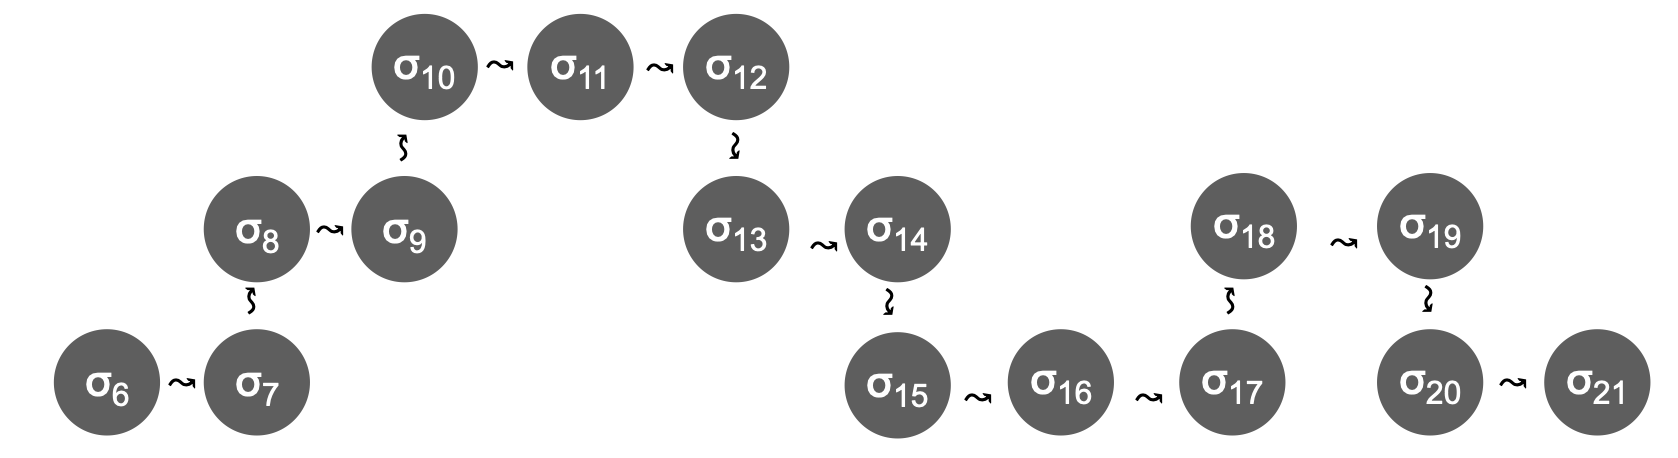
\includegraphics[width=\linewidth]{diagrams/bounded.png}
} 
 \\
\hline
%\begin{tabular}{lclclclcl}
%$\leadstoOrig  {\Mtwo} {\sigma_8}    {\sigma_9} $  & & 
%$\leadstoOrig  {\Mtwo} {\sigma_9}    {\sigma_{10}} $ &  &
%$\leadstoOrig  {\Mtwo} {\sigma_{12}}   {\sigma_{13}} $ & & 
%$\leadstoOrig  {\Mtwo} {\sigma_{13}}    {\sigma_{14}} $  &  &
%$\leadstoOrig {\Mtwo}{\sigma_{14}}   {\sigma_{15}} $
%\\
%\hline
%$\leadstoOrigStar  {\Mtwo} {\sigma_8}   {\sigma_{12}}$ & & \ & & \ & & $\leadstoOrigStar  {\Mtwo} {\sigma_{10}}   {\sigma_{15}}$
%\\
%\hline
%\end{tabular}
%\\
%\hline
\end{tabular}
   \caption{Illustrating   $\leadstoOrig  {\Mtwo} {\sigma}    {\sigma'}$ 
    }
   \label{fig:UpSemantics}
 \end{figure}
 
%\susan{I don't think the two lines at the bottom of the figure are needed here and in the next figure. \sdN{agree, but highlight.}} 
 
%{Note that $\leadstoOrig {\Mtwo}{\sigma_{8}}   {\sigma_{9}} $ and $\leadstoOrig {\Mtwo}{\sigma_{13}}   {\sigma_{14}} $ are steps within the same call, but 
%$\leadstoOrig {\Mtwo}{\sigma_{14}}   {\sigma_{15}} $ and $\leadstoOrig {\Mtwo}{\sigma_{17}}   {\sigma_{18}} $ are not. %steps within the same call,
%% even though all four states ($\sigma_{13}$, $\sigma_{14}$, $\sigma_{17}$, and $\sigma_{18}$), have the same number of frames on their stack.
%We want a semantics to reflect whether execution steps happen within the bounds of certain call. For this, we define \emph{bounded execution}, 
%$\leadstoBounded {\Mtwo} {\sigma} {\sigma''} {\sigma'}$ 
%which are execution steps which lead from $\sigma$ to $\sigma'$ while not popping  $\sigma''$-s top frame.
%This will be defined in Section \ref{sect:bounded}.
%}

\subsection*{Applicability} 
While our work is based on the particular language  \LangOO , % a simple, imperative, typed, object oriented  language with unforgeable addresses and private fields, we believe that % our approach
we believe that it is applicable to several programming paradigms, and  that   unforgeability and privacy
 can be replaced  by lower level mechanisms such as capability machines \cite{vanproving,davis2019cheriabi}.


\section{From \LangOO to \AssertLang}

{To develop the semantics of our assertions language, \AssertLang, we   build three auxiliary concepts on  top of  \LangOO: bounded execution, method calls and returns, and reachable objects.}


\subsection{Bounded Execution}
\label{sect:bounded}

{The semantics from the earlier section allows arbitrary numbers of method calls and returns. 
In particular it is possible to start with a state $\sigma$ and perform more returns than calls --
\eg $\leadstoOrigStar  {\Mtwo} {\sigma_{8}}   {\sigma_{15}}$. 
\sdN{In the sense of $\leadsto^*$,  the state $\sigma_{15}$  is one of the    ``future'' states for $\sigma_8$.}

\sdN{This  is  is a perfectly natural semantics, 
but for the purposes of our work, we need a notion of  ``future state'' which  includes method calls and returns, but does not
include returns from the currently executing method -- \cf Def. \ref{def:necessity-semantics}(2).}
Thus,
the future states of $\sigma_8$  only include 
 % states which are being visited as a result of  executing $\sigma_8$'s top continuation}; that is, it includes the states 
 $\sigma_9$, $\sigma_{10}$, $\sigma_{11}$, $\sigma_{12}$, $\sigma_{13}$, and $\sigma_{14}$, but \emph{not} $\sigma_{15}$ \sdN{-- the latter results from returning from $\sigma_{8}$'s top continuation.}
% since $\sigma$'s top frame will have been popped before we reach $\sigma'$. 

To obtain this  notion of future, we define  execution from the viewpoint of an original state, $\sigma_o$, which  is ``bounded'' so as not to ever pop   $\sigma_o$'s top frame :


 
\begin{definition}[Bounded Execution]
\label{def:shallow:term}
We define relations \  {\red{ $\leadstoBoundedThree {\Mtwo} {\sigma} {\sigma_o} {\sigma'}}$}\ and\  $\leadstoBounded  {\Mtwo} {\sigma} {\sigma'}$ as:

\begin{itemize}
\item
 $\leadstoBoundedThree {\Mtwo} {\sigma} {\sigma_o}  {\sigma'}$ \ \  iff \ \ \  $\leadstoOrig {\Mtwo} {\sigma} {\sigma'} % $\\
% $\strut  \hspace{3.6cm}\ 
\ \  \wedge $\\
$\strut  \hspace{2.9cm}\ \  \ \ \   \exists \phi,\psi, \psi_1, \psi_2.[ \ \sigma_o = (\phi\cdot\psi,\_) \ \wedge \ \sigma = (\psi_1\cdot \psi, \_)
\ \wedge\ \sigma' = (\psi_2\cdot \psi, \_)\ ] $ 
\item
 $\leadstoBoundedStarThree  {\Mtwo}  {\sigma}  {\sigma_o} {\sigma'}$\ \  iff \ \ $\sigma=\sigma'\ \ \vee$\\
$\strut  \hspace{3cm}\ \ \exists n\!\in\!\mathbb{N},\sigma_0,..,\sigma_n.[\ \forall i\!\! \in\!\! [0..n).\leadstoBoundedThree {\Mtwo}  {\sigma_i}  {\sigma_o} {\sigma_{i+1}} \ \wedge\ \sigma=\sigma_0\ \wedge\ \sigma'=\sigma_n\ ]$
 \item
\sdN{  $\leadstoBounded  {\Mtwo} {\sigma}   {\sigma'}$\ \  \ \ \ \ \ \   \ \ \ \ iff \ \ \ $\leadstoBoundedThree {\Mtwo} {\sigma} {\sigma}  {\sigma'}$}
  \item
\sdN{  $\leadstoBoundedStar {\Mtwo}  {\sigma}  {\sigma'}  $\ \ \ \ \ \ \ \ \   \ iff \ \ \ $\leadstoBoundedStarThree {\Mtwo}  {\sigma}  {\sigma} {\sigma'}$}\ \  
\end{itemize}
\end{definition}
 

We continue with  Fig. \ref{fig:UpSemantics}. Here $\leadstoOrig {\Mtwo} {\sigma_{14}}  {\sigma_{15}}$ 
 but    $\notLeadstoBoundedThree {\Mtwo}  {\sigma_{14}} {\sigma_{14}} {\sigma_{15}}$
and  $\notLeadstoBounded  {\Mtwo}  {\sigma_{14}}   {\sigma_{15}}$
--  this step would pop  $\sigma_{14}$'s
 top frame. 
% Therefore,   $\leadstoOrigStar {\Mtwo} {\sigma_8}  {\sigma_{15}}$ 
%  but  $\notLeadstoBoundedStarThree {\Mtwo} {\sigma_8} {\sigma_8} {\sigma_{15}}$, and  $\notLeadstoBoundedStarThree {\Mtwo}  {\sigma_8} {\sigma_{15}}$.
 Also, $\leadstoOrigStar {\Mtwo} {\sigma_8}  {\sigma_{18}}$ 
 but  $\notLeadstoBoundedStar {\Mtwo} {\sigma_8}   {\sigma_{18}}$  -- even though $\sigma_8$ and $\sigma_{18}$ have the same depth of stack, they belong to different calls.
 
 %\begin{figure}[htb]
%\begin{tabular}{|c|}
% \hline %  \\ -- this added one vertical space
%\resizebox{7cm}{!}{
%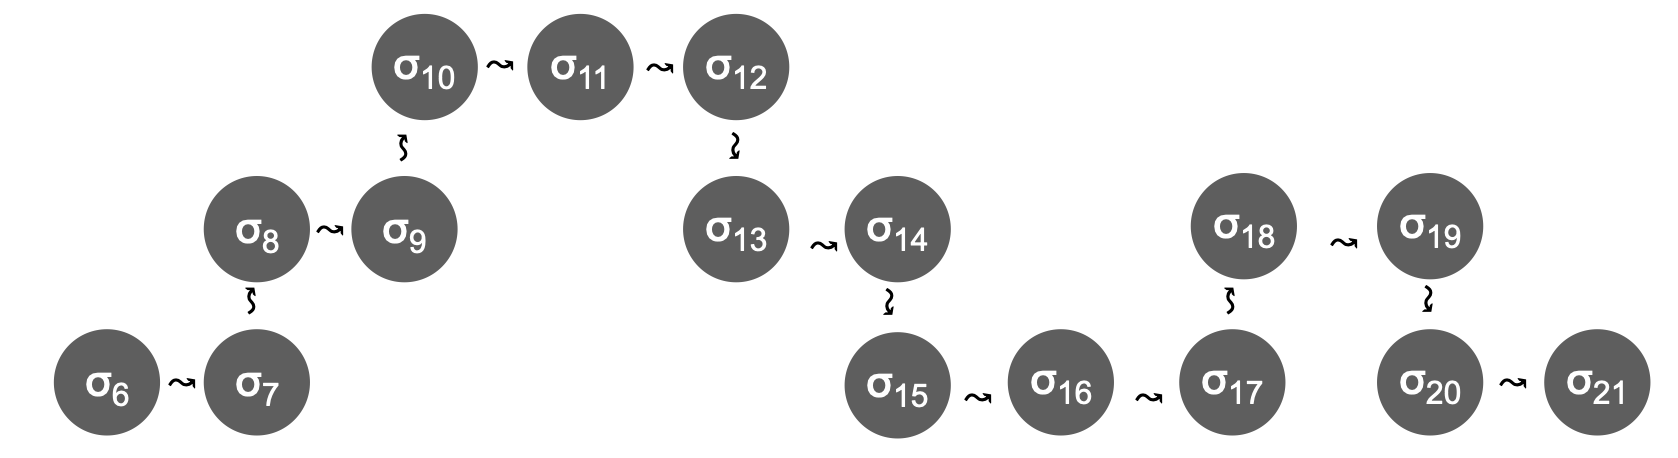
\includegraphics[width=\linewidth]{diagrams/bounded.png}
%} 
% \\
%\hline
%\begin{tabular}{lclclclclcl}
% $\leadstoBoundedThree  {\Mtwo} {\sigma_{12}} {\sigma_8}  {\sigma_{13}} $  & &   $\leadstoBoundedThree {\Mtwo} {\sigma_{13}}  {\sigma_{8}}  {\sigma_{14}} $ &  & \leadstoBoundedStar   {\Mtwo}   {\sigma_8}  {\sigma_{14}}  & &
%$\notLeadstoBoundedThree  {\Mtwo} {\sigma_{14}} {\sigma_8}  {\sigma_{15}} $ & &  
%\\
%\end{tabular}
%\\
%\hline
%\end{tabular}
%   \caption{Illustrating   $\leadstoBoundedThree  {\Mtwo} {\sigma}  {\sigma_o} {\sigma'}$, and $\leadstoBounded {\Mtwo} {\sigma}   {\sigma'}$}
%   \label{fig:UpSemanticsBounded}
% \end{figure}

%  \vspace{.1cm}
 
\sdN{Bounded semantics impose restrictions on the set of future states, but only from the viewpoint of
\red{some}
%a given 
origin state (\cf Lemma \ref{lemma:orig:to:bounded}):  
\red{Executions starting at  initial states are bounded  -  \cf part (\ref{otbOne}).}
\red{While $ \notLeadstoBoundedStar {\Mtwo} {\sigma}  {\sigma'}$ expresses that $\sigma'$ is not part of the "bounded" future of $\sigma$, if, in addition, $\leadstoOrigStar {\Mtwo} {\sigma_{init}}  {\sigma}  \ \wedge\ \leadstoOrigStar {\Mtwo} {\sigma}  {\sigma'}$ holds, then 
 $\sigma$ and $\sigma'$ are  in $\sigma_{init}$'s bounded future, and  from $\sigma_{init}$'s viewpoint, $\sigma'$ is a transitive bounded successor of $\sigma$ - \cf  part (\ref{otbTwo}).
Finally,  part (\ref{otbThree})  genaralizes %  Lemma \ref{lemma:orig:to:bounded}, 
part (\ref{otbTwo}).}}
% there exists a further, earlier, state $\sigma_o$, such that both $\sigma$ and $\sigma'$ are  
%part   of $\sigma_o$'s bounded future. Moreover, from $\sigma_o$'s viewpoint, $\sigma'$ is a transitive bounded successor of $\sigma$.}

\sdN{\begin{lemma}
\label{lemma:orig:to:bounded}
For all $\overline M$, all $n,m\in \mathbb{N}$ with $m\leq n$, $\sigma_0$, ... $\sigma_n$,  $\sigma_{init}$, $\sigma$, $\sigma'$, where
$\sigma_{init}$ is initial:\footnote{An \emph{Initial} state's heap contains a single object of class \prg{Object}, and
its  stack   consists of a single frame, whose local variable map is a
mapping from \prg{this} to the single object, and whose continuation is  any statement.
(See Definition %s \ref{def:initial} and 
\ref{def:arising} and the 
{appendices %of the full paper 
\cite{necessityFull}).}} 
\begin{enumerate} 
\item 
\label{otbOne}
$\leadstoOrigStar {\Mtwo} {\sigma_{init}}  {\sigma}\ \ \Longrightarrow\ \  \leadstoBoundedStar {\Mtwo}  {\sigma_{init}} {\sigma}$.
\item 
\label{otbTwo}
$\leadstoOrigStar {\Mtwo} {\sigma_{init}}  {\sigma}\ \wedge\ \leadstoOrigStar {\Mtwo} {\sigma}  {\sigma'}\ \ \Longrightarrow\ \  \leadstoBoundedStarThree {\Mtwo} {\sigma} {\sigma_{init}} {\sigma'}$.
%there exists a $\sigma_o$, such that $\leadstoBoundedStar {\Mtwo} {\sigma_{init}}  {\sigma_o}$, and
% $\leadstoBoundedStar {\Mtwo} {\sigma_o}  {\sigma}$, and $\leadstoBoundedStar {\Mtwo} {\sigma_o}  {\sigma'}$, and $\leadstoBoundedStar {\Mtwo} {\sigma_o}  {\sigma'}$. More specifically, 
% $\leadstoBoundedStarThree {\Mtwo} {\sigma} {\sigma_o} {\sigma'}$.
\item
\label{otbThree}
 $\forall i\!\in\! [0..m).\ \leadstoOrig  {\Mtwo} {\sigma_{i}}  {\sigma_{i+1}}\ \wedge\ \sigma_{init}=\sigma_0$ \\
 % \ \wedge \  \sigma=\sigma_m \ \wedge\ \sigma' =\sigma_n  $ \\
\strut \hspace{0.5cm} $\ \ \Longrightarrow \ \  \exists k\leq n.[\ \ \ \forall i\leq k.[\  \leadstoBoundedStar  {\Mtwo}   {\sigma_{init}} {\sigma_i}\ \wedge \ \leadstoBoundedStarThree  {\Mtwo}  {\sigma_m}  {\sigma_{i}} {\sigma_n} ]\ \ \  \wedge$\\
\strut \hspace{3cm} $ \forall i> k. [\  \notLeadstoBoundedStarThree  {\Mtwo}  {\sigma_m}  {\sigma_{i}} {\sigma_n}\ ] \ \ \ ]$.
\end{enumerate} 
\end{lemma}
}

 
\subsection{Method Calls and Returns}


{External calls are a central consideration of our work, therefore  the point at which a method is called or returned from is of particular importance. 
The operator $\pushSymbol$ describes both call and return:
% pushing a new frame on the stack: 
 $ \PushS  {\alpha} {\sigma} $ is  the set of states obtained by pushing onto the stack of $\sigma$ a new frame with some continuation  and a local variable map \sdN{whose domain has the same cardinality as $\overline \alpha$ and whose range  is} $\overline \alpha$, while leaving the heap unmodified.
The elements of $ \PushS  {\alpha} {\sigma} $ only differ in the identifiers in the local variable map, as well as the continuation  of the top frame. 
}

\begin{definition}
\label{def:push:frame}
Given a state $\sigma$, addresses $\overline \alpha$, and variables or addresses $\overline \va$, we define
\begin{itemize}
\item
$ \PushS  {\alpha} {\sigma} \ =\ \{ \ \sigma' \ \mid\ \sigma=(\psi, \chi)\  \wedge\  (\phi\cdot \psi, \chi) \ \wedge\ rng(\phi)=\overline \alpha \ \ \mbox{ for some } \phi, \psi, \chi \ \}$
\item
{$ \PushS  {\va}  {\sigma}$ is short for  $ \PushS  {\interpret {\sigma} {\va}} {\sigma} $.}
\end{itemize}
\end{definition}

 {Lemma \ref{lemma:push} below says that  $\pushSymbol$ characterizes  calls and returns.  (\ref{pushOne}):\ $ \PushS   {\alpha} {\sigma}$ describes    direct successor states of  a $\sigma$ with a continuation which calls a method with receiver and arguments $\overline \alpha$. 
 (\ref{pushTwo}):\ $ \PushS   {\alpha} {\sigma'}$  describes direct predecessor states of  a $\sigma'$ with ground continuation.}
  
\begin{lemma}% [$\pushSymbol$  for calls and returns]
\label{lemma:push}
For all states $\sigma$, $\sigma'$, modules $\Mtwo$, and addresses $\overline \alpha$. If \ $\leadstoOrig {\Mtwo} {\sigma}   {\sigma'} $, \ then 
\begin{enumerate}
\item
\label{pushOne}
$\sigma'\in   \PushS  {\alpha} {\sigma}  \ \ \Longleftrightarrow \ \ 
\exists x, m, \overline{y}.[\ \ \sigma.\prg{cont} \txteq x:=y_0.m(y_1,...y_n); \_\ \ \wedge \ \
{\overline { \interpret  \sigma y}} = \overline \alpha \ ] $
\item
\label{pushTwo}
$\sigma\in   \PushS  {\alpha} {\sigma'}  \ \ \Longleftrightarrow \ \ \exists x, \alpha'.[\ \  \sigma'.\prg{cont}\txteq x:=\alpha';\_ \ \ \wedge \ \  \sigma.\prg{cont}\txteq\alpha'\  ] $
\end{enumerate}

\end{lemma}

 

 {Consider Fig. \ref{fig:UpSemantics} again: $\sigma_8\in   \PushS  {\alpha} {\sigma_7}$ for some $\overline \alpha$, and 
 $\sigma_{14}\in\PushS  {\alpha'} {\sigma_{15}}$ for some $\overline \alpha'$. Namely, $\sigma_8$ is the first state right after calling a method with receiver and
 arguments $\overline \alpha$ and $\sigma_{14}$ is the last state before returning from that method call back to $\sigma_{15}$.
Note that $\overline \alpha$ may differ from $\overline \alpha'$, because between $\sigma_8$ and $\sigma_{15}$ there may 
have been assignments to local variables -- only the receiver will have remained the same.
Similarly, 
 $\sigma_{10}\in\PushS  {\alpha''} {\sigma_9}$ for some $\overline \alpha''$, and  $\sigma_{12}\in\PushS  {\alpha'''} {\sigma_13}$ for some $\overline \alpha'''$, etc.
}


  \subsection{{Reachable  Objects}}

 {A central concept to our work is object \emph{protection}, which we will define in   Sect. \ref{sect:protect}: It requires that no external object  
reachable from the top frame  can have unmitigated access to that object.}
%
%{The  \SpecLang  specifications support universal quantification over  objects; such specifications 
%are applicable  to all objects in the heap witch, are however, either locally reachable (i.e. there is in the heap a path from the an 
%object on the top frame to the particular object), or globally reachable (i.e. there is in the heap a path from the an 
%object on some frame to the particular object.)
%%In this section  we will formally define these concepts.}\footnoteSD{TODO we need a better motivation for these concepts.}
%
An object $\alpha$ is  locally reachable, $ \LRelevant \alpha \sigma $, if it is reachable from the top frame on the stack of $\sigma$,
and it is globally reachable, $\GRelevant \alpha \sigma$, if it is reachable from from any  frame on the stack of $\sigma$.
 
\begin{definition} We define 
\begin{itemize}
\item
$ \LRelevant \alpha \sigma $ \ \ iff\ \  
$\exists \phi.[\ \sigma=(\phi\cdot\_, \_)$ and $\Relevant \alpha \phi \sigma\ ]$. % for some $\phi$
\item
$\GRelevant \alpha \sigma$  \ \ iff\ \  
$\exists \phi.[\ \sigma=(\_\cdot\phi\cdot\_, \_)$ and $\Relevant \alpha \phi \sigma\ ]$. % for some $\phi$
\end{itemize}
where\\
$\strut\ \ \ \  \ \ \ \ \ \ \Relevant \alpha \phi \sigma $  \ \ \ \ \ \ \ iff\ \  
$\exists n\in \mathbb{N}.\exists \prg{f}_1,... \prg{f}_n.\exists \prg{x}.[ \ \interpret{\sigma}{\phi(x).\prg{f}_1.....\prg{f}_n} = \alpha \ \ ]$.

\end{definition}

 \begin{figure}[htb]
\begin{tabular}{|c|c|c|}
\hline \\
\resizebox{3.5cm}{!}{
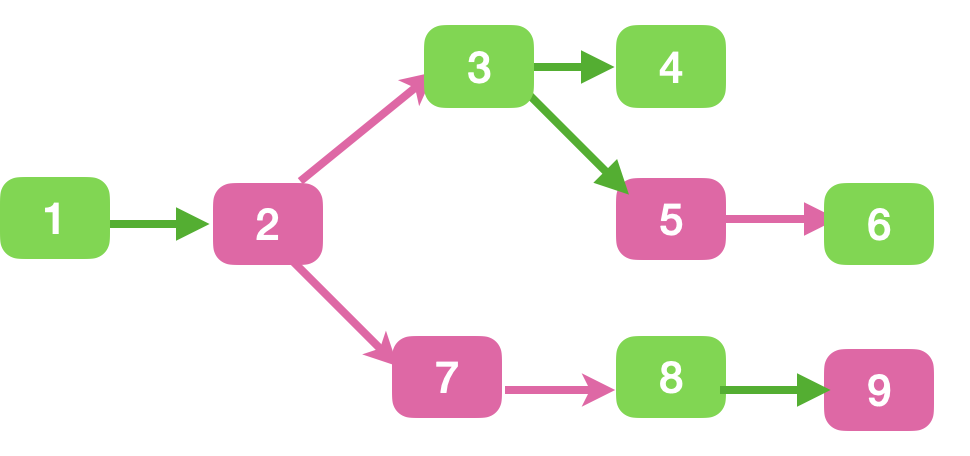
\includegraphics[width=\linewidth]{diagrams/heap.png}
} 
&
\resizebox{5cm}{!}{
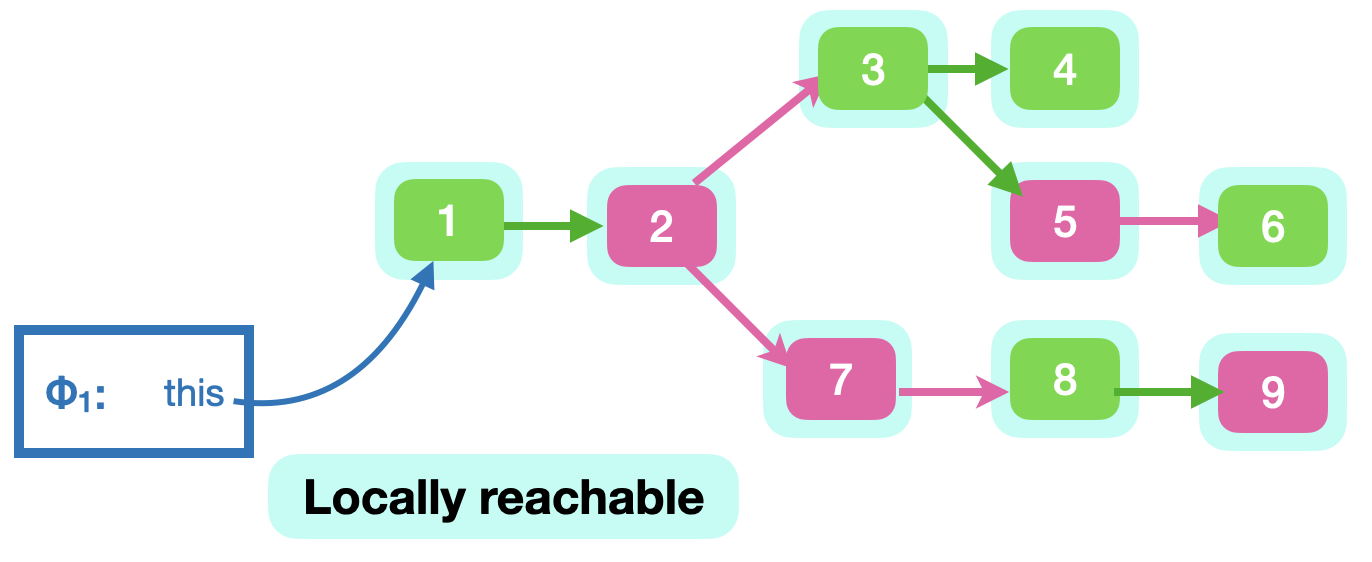
\includegraphics[width=\linewidth]{diagrams/locReachA.png}
} 
&
\resizebox{5cm}{!}{
\includegraphics[width=\linewidth]{diagrams//locReachb.png}
} 
\\
\hline
 a heap
&
Locally Reachable from $\phi_1$
&
Locally Reachable from $\phi_2$
\\
\hline \hline
\end{tabular}
   \caption{A heap, and Locally Reachable Objects. % from $\phi_1$ and $\phi_2$. 
   The distinction of objects into  green or pink is explained in later chapters}
   \label{fig:LReachable}
 \end{figure}

We illustrate these concepts in Fig. \ref{fig:LReachable}: In the middle pane the top frame is $\phi_1$ which maps \prg{this} to $o_1$; all objects are locally reachable. 
In the right pane the top frame is $\phi_2$, which maps \prg{this} to $o_3$, and $x$ to $o_7$; now $o_1$ and $o_2$ are no longer locally reachable.

Lemma  \ref{lemma:relevant} % describes properties of global reachability. 
says that  (\ref{oneGR}) Locally reachable objects are globally reachable. 
(\ref{twoGR}) 
% Any object which will be globally reachable at some future state  and which exists object in the current state, is globally reachable the current state: that is, 
Globally unreachable objects may not become reachable in the future.
\footnoteSD{cite "only connectivity begets connectivity"}
(\ref{oneLR}) A locally reachable object  after a call was also locally reachable before the call.
(\ref{threeLR}) A pre-existing object, locally reachable  object after a any number of bounded execution steps, was locally reachable at the first step.


\begin{lemma}
\label{lemma:relevant}
For all module sets $\Mtwo$, states $\sigma$, $\sigma'$,   objects $o$, and $\overline o$:\footnoteSD{{TODO decide whether $o$ or $\alpha$}}
%and  variables ${\overline z}$, and statements $s:$
\begin{enumerate}
\item
\label{oneGR}
$ \LRelevant o \sigma\ \ \Longrightarrow \ \   \GRelevant o \sigma$
\item
\label{twoGR}
${\leadstoOrigStar {\Mtwo}  {\sigma}  {\sigma'}} \ \ \wedge \ \  \GRelevant o {\sigma'} \ \ \wedge\ \  {o\in \sigma} \ \ \ \Longrightarrow \ \  \ \GRelevant o {\sigma}$.
\item
\label{oneLR}
{$\sigma'\in \PushS {o} {\sigma}  \ \ \wedge \ \  \LRelevant {\overline o} {\sigma} \ \ \wedge\ \   \LRelevant o {\sigma'} \ \ \ \Longrightarrow \ \ \  \LRelevant o {\sigma}$
}
\item
\label{threeLR}
${\leadstoBoundedStar {\Mtwo}  {\sigma}    {\sigma'}} \ \ \wedge \ \   \LRelevant o {\sigma'}\  \ \wedge\ \  {o\in \sigma} \ \ \ \Longrightarrow \ \ \ \LRelevant o {\sigma}$.
\end{enumerate}
\end{lemma}

{Consider Fig.  \ref{fig:UpSemantics}. %, and Fig.  \ref{fig:UpSemanticsBounded}.
Lemma \ref{lemma:relevant}.\ref{threeLR}  promises that any objects locally reachable in $\sigma_{14}$ which already existed in $\sigma_{8}$, were locally reachable in $\sigma_{8}$. However, the lemma is only  applicable to bounded execution, and as 
$\notLeadstoBoundedStar {\Mtwo} {\sigma_8}  {\sigma_{17}}$, 
the lemma does not promise that  objects locally reachable in $\sigma_{17}$ which already existed in $\sigma_{8}$, were locally accessible in $\sigma_{8}$ -- namely it could be that objects are made globally reachable upon method return, during the step from $\sigma_{14}$ to $\sigma_{15}$.}


